\chapter{Ciclo de Vida do Sistema}
\section{Definição da Abordagem e Metodologia}
Foi definida a utilização de uma abordagem de desenvolvimento ágil \cite{beck2001agile} para o contexto inicial do projeto, levando-se em conta que o processo de desenvolvimento seria realizado pelo próprio autor, a disponibilidade do cliente seria mais abrangente e o projeto evoluiria aos poucos, com entregas contínuas de pequenos incrementos de \textit{software}.

A metodologia utilizada se baseou no Kanban \cite{radigan_2015}, com algumas práticas do \textit{Extreme Programming}, visto que ambos atendiam de maneira adequada ao fluxo de trabalho contínuo, previsto pela abordagem escolhida.

Para auxiliar nas \textit{releases} do projeto, foi utilizado o conceito de \textit{sprints}, provido pelo \textit{Scrum} \cite{scrum_guide}. As \textit{sprints} são pequenos intervalos de tempo, de um mês ou menos, durante o qual uma versão incremental potencialmente utilizável do produto é criada. Uma nova Sprint se inicia imediatamente após a conclusão da Sprint anterior. O projeto adotou \textit{sprints} de 2 semanas.

Ressalta-se que os próximos tópicos do ciclo de vida não foram realizados completamente em sequência, visto que esses acabavam se intercalando em determinados momentos, como previsto em uma abordagem ágil.

\section{Contexto e Necessidades}
A Prefeitura de Campus designou dois professores doutores da Faculdade UnB Gama, Alex Reis e Loana Nunes Valesco, para darem suporte às necessidades energéticas que o sistema deveria atender. Por questões de disponibilidade e quantidade de equipamentos de medição adquiridos, o campus UnB Gama foi escolhido como ambiente de teste para a primeira parte do projeto.

Tendo como problema a falta de monitoramento energético adequado na Universidade de Brasília, foi realizado um estudo mais aprofundado sobre o contexto para identificar as necessidades do cliente. Tal estudo abordou fatores energéticos cruciais, como por exemplo, sistemas trifásicos, horários de ponta e fora de ponta, tensão, corrente, resistência e afins.

A energia elétrica em corrente alternada e em sistema trifásico é um dos métodos mais comuns para se gerar, transmitir e distribuir corrente elétrica alternada. Baseia-se em um sistema denominado polifásico e empresas elétricas de todo o mundo o utilizam como meio de transmissão de energia \cite{stevenson_1962}.

A Tarifa Branca sinaliza a variação do valor da energia conforme o dia e o horário do consumo. Nos dias úteis, o valor da Tarifa Branca varia em três horários: ponta, intermediário e fora de ponta. Na ponta e no intermediário, a energia é mais cara. Fora de ponta, é mais barata. Durante feriados nacionais e fins de semana, o valor é sempre fora de ponta \cite{aneel}.

Com um entendimento melhor do contexto e reuniões com os professores, as seguintes necessidades foram encontradas:

\begin{itemize}
    \item Cada campus da Universidade de Brasília deve ser responsável por realizar seu próprio monitoramento energético;
    \item O campus Darcy Ribeiro deve funcionar como uma espécie de administração central, capaz de reunir os dados de todos os outros campus;
    \item As medições devem ser armazenadas e analisadas.
\end{itemize}

Inicialmente, o nome do projeto foi definido como Sistema de Monitoramento Energético - Universidade de Brasília (SME-UnB), porém, após algumas reuniões realizadas, percebeu-se a possiblidade de monitoramento, no futuro, de medições de água. Tendo em vista os recursos que seriam monitorados, o nome do projeto foi modificado para Sistema de Monitoramento de Insumos - Universidade de Brasília (SMI-UnB).

Foi definido que, para o contexto inicial do projeto, seriam enfatizados os dados de energia e que seriam entregues duas \textit{releases}, de aproximadamente 80 dias, sendo estas:

\begin{itemize}
    \item Release 1: coleta dos dados de energia;
    \item Release 2: apresentação dos dados e protótipo de comunicação inter-campi.
\end{itemize}

Foi escolhido o \textit{software} livre GitLab CE\footnote{\url{https://gitlab.com/gitlab-org/gitlab-ce}} para realizar a hospedagem do código/documentação do projeto\footnote{\url{https://gitlab.com/brenddongontijo/SMI-UnB}} e o controle de mudanças. Já para o controle de versão, definiu-se a utilização da ferramenta Git\footnote{\url{https://git-scm.com/}}.

A escolha do GitLab CE se deve pela cultura de \textit{software} livre, por se tratar de um projeto de âmbito acadêmico e público. Assim, o compartilhamento de conhecimento pode ser realizado de maneira mais fácil e a qualidade final não seria comprometida \cite{raymond1999}.

A licença escolhida para o projeto foi a MIT\footnote{\url{https://opensource.org/licenses/MIT}}. Criada pelo \textit{Massachusetts Institute of Technology}, a licença MIT é bastante utilizada pelo meio acadêmico por sua facilidade de implantação e permissividade, autorizando o uso comercial, modificação, distribuição e sublicenciamento \cite{mit_license}.

A UnB não possui um modelo de referência para o licenciamento de \textit{software} livre. Assim, a licença escolhida foi adequada, pois prevê a possibilidade de sublicenciar o projeto no futuro, caso seja necessário.

\section{Requisitos}
Os requisitos do projeto foram adquiridos através das reuniões e mapeados, de maneira mais simplificada, em \textit{milestones} \cite{gitlab} no repositório. Cada \textit{milestone} possuía um conjunto de \textit{issues} associadas, as quais apresentariam uma terminologia mais técnica da solução em si.

Uma \textit{milestone} funciona como um quadro Kanban, tendo as colunas \textit{To Do}, \textit{Doing} e \textit{Done}. Pode possuir uma data início/fim e é composta por um aglomerado de problemas, comumente chamados de \textit{issues}, os quais ficam transitando pelas colunas, conforme necessário.

As \textit{milestones} e \textit{issues} foram criadas no decorrer do projeto, ou seja, a cada \textit{sprint} foram avaliadas as mudanças de escopo ocorridas, quais seriam as \textit{issues} da próxima \textit{sprint}, se era necessário criar ou atualizar uma determinada \textit{milestone}, etc. As \textit{milestones} do projeto, Figura \ref{milestones}, foram divididas da seguinte maneira:

\begin{itemize}
    \item \textit{Bugfixes} GPP/MDS: refatorações sobre o incremento de \textit{software} adquirido por uma equipe externa de desenvolvedores e gerentes, esta equipe será explicada na próxima sub-sessão. A refatoração abordava arrumar todo o sistema de login e de usuários, criando diferentes tipos de acesso e algumas permissões importantes;
    \item Coleta de dados transdutor de energia: gerência de transdutores de energia e coleta de suas informações, interfaciando seus protocolos de transporte e serial. Definição de validações sobre a gerência, armazenamento de transdutores, criação/leitura das mensagens seriais e envio/recebimento dos pacotes presentes na camada de transporte;
    \item Sistema de Gráficos: gráfico de linhas dinâmico para apresentação das medições realizadas por um transdutor, contendo pontos de máximo/mínimo, opções para geração do gráfico, marcações para períodos com ausência de medições. Além do gráfico, definiu-se uma refatoração sobre todo o \textit{layout} do sistema;
    \item Campus e Edifícios: mapeamento de como a UnB seria estruturada na aplicação, definição de toda a gerência e validação dos \textit{campi}, edifícios e integração com a gerência de transdutores;
    \item Transmissão de Dados Entre Servidores: definição de servidores com papéis de mestre e escravo, API \textit{web} capaz de se comunicar com sistemas externos, construção de um ambiente propício a ser de produção, protótipo de comunicação entre administração central e \textit{campi} da UnB.
\end{itemize}

\begin{figure}[!htb]
    \centering
    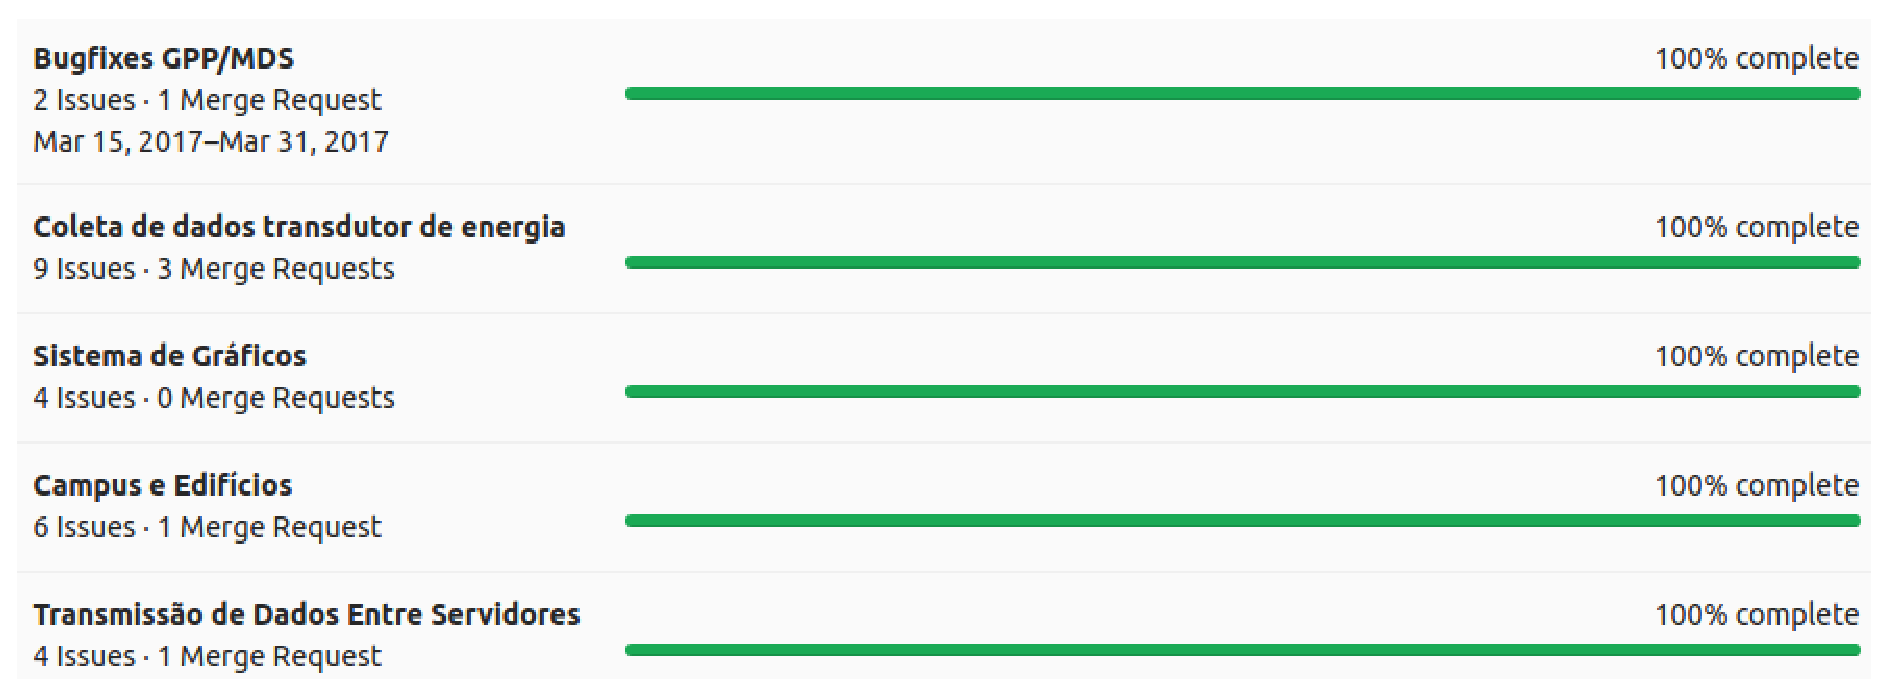
\includegraphics[keepaspectratio=true,scale=0.51]{figuras/milestones.eps}
    \caption{\textit{Milestones} realizadas durante as duas \textit{releases} do projeto.}
    \label{milestones}
\end{figure}

\section{Visão Geral do Desenvolvimento}
O desenvolvimento da parte inicial do projeto foi marcado por duas \textit{releases}, sendo estas:

\begin{itemize}
    \item \textit{Release} 1: 20/07/2016 a 25/11/2016;
    \item \textit{Release} 2: 06/03/2017 a 23/06/2017.
\end{itemize}

\subsection{\textit{Release} 1}
A primeira \textit{release} teve início com um estudo aprofundado sobre o equipamento de medição de energia que seria utilizado. Após o estudo, foi definida a arquitetura inicial do projeto e realizado um pequeno protótipo funcional, Figuras \ref{dados02} e \ref{dados01}, que conseguia efetivamente coletar os dados de energia.

\begin{figure}[!htb]
    \centering
    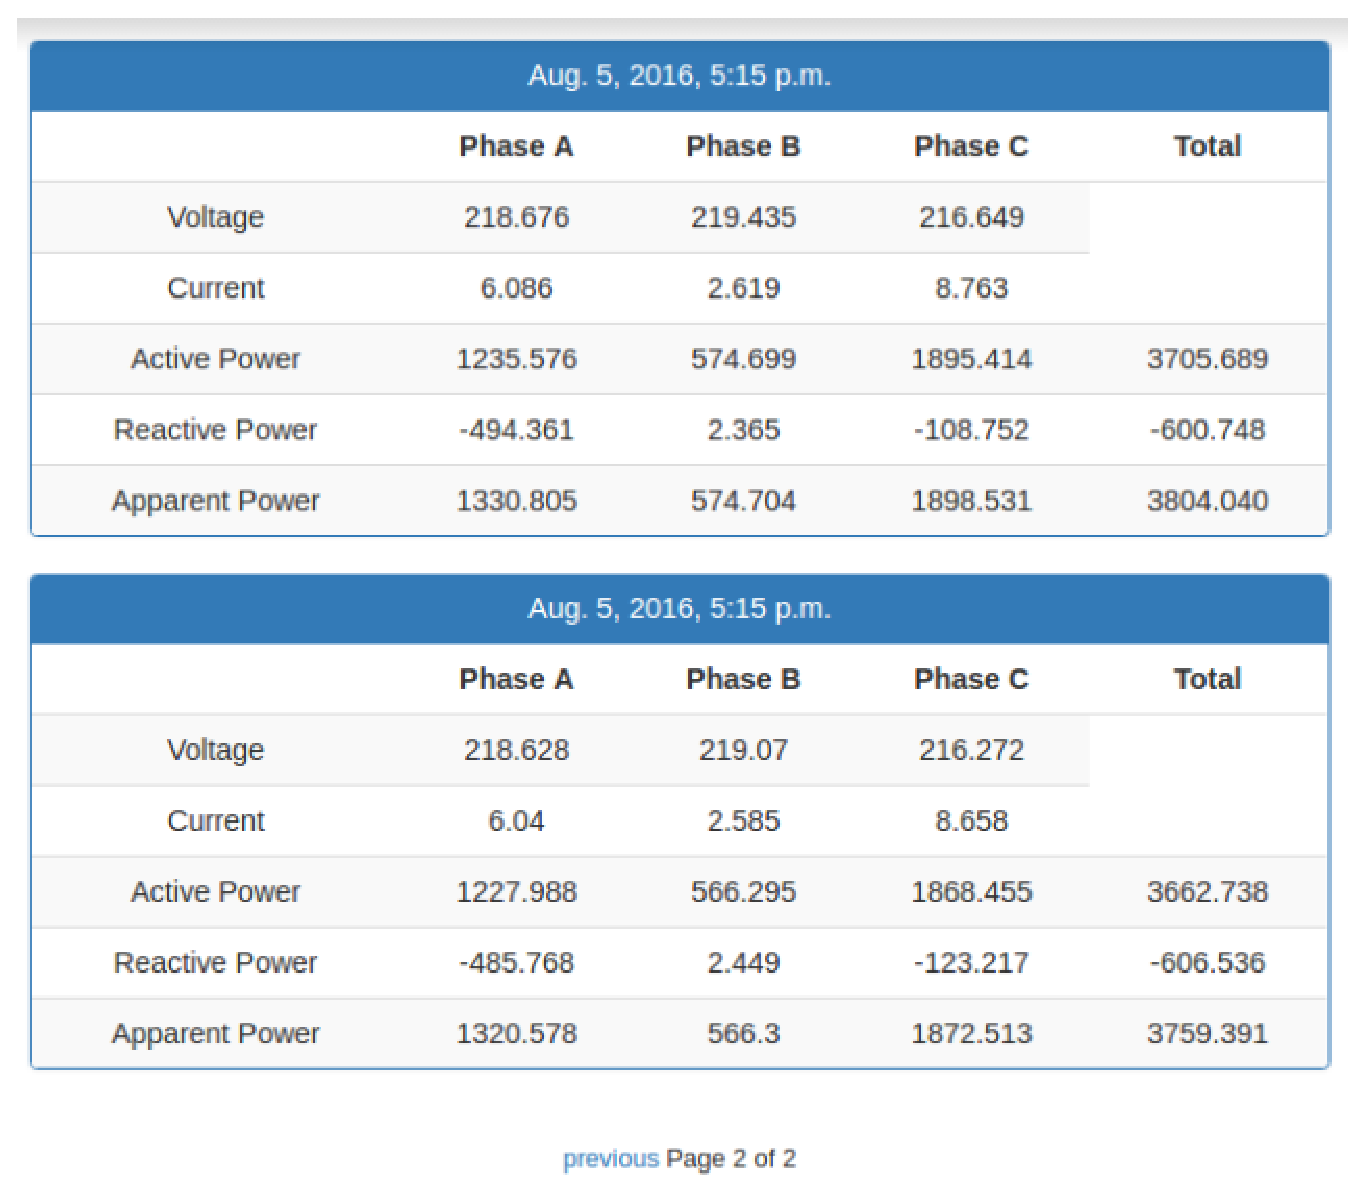
\includegraphics[keepaspectratio=true,scale=0.5]{figuras/coleta_dados_02.eps}
    \caption{Protótipo para apresentação dos transdutores \textit{release} 1.}
    \label{dados02}
\end{figure}

\begin{figure}[!htb]
    \centering
    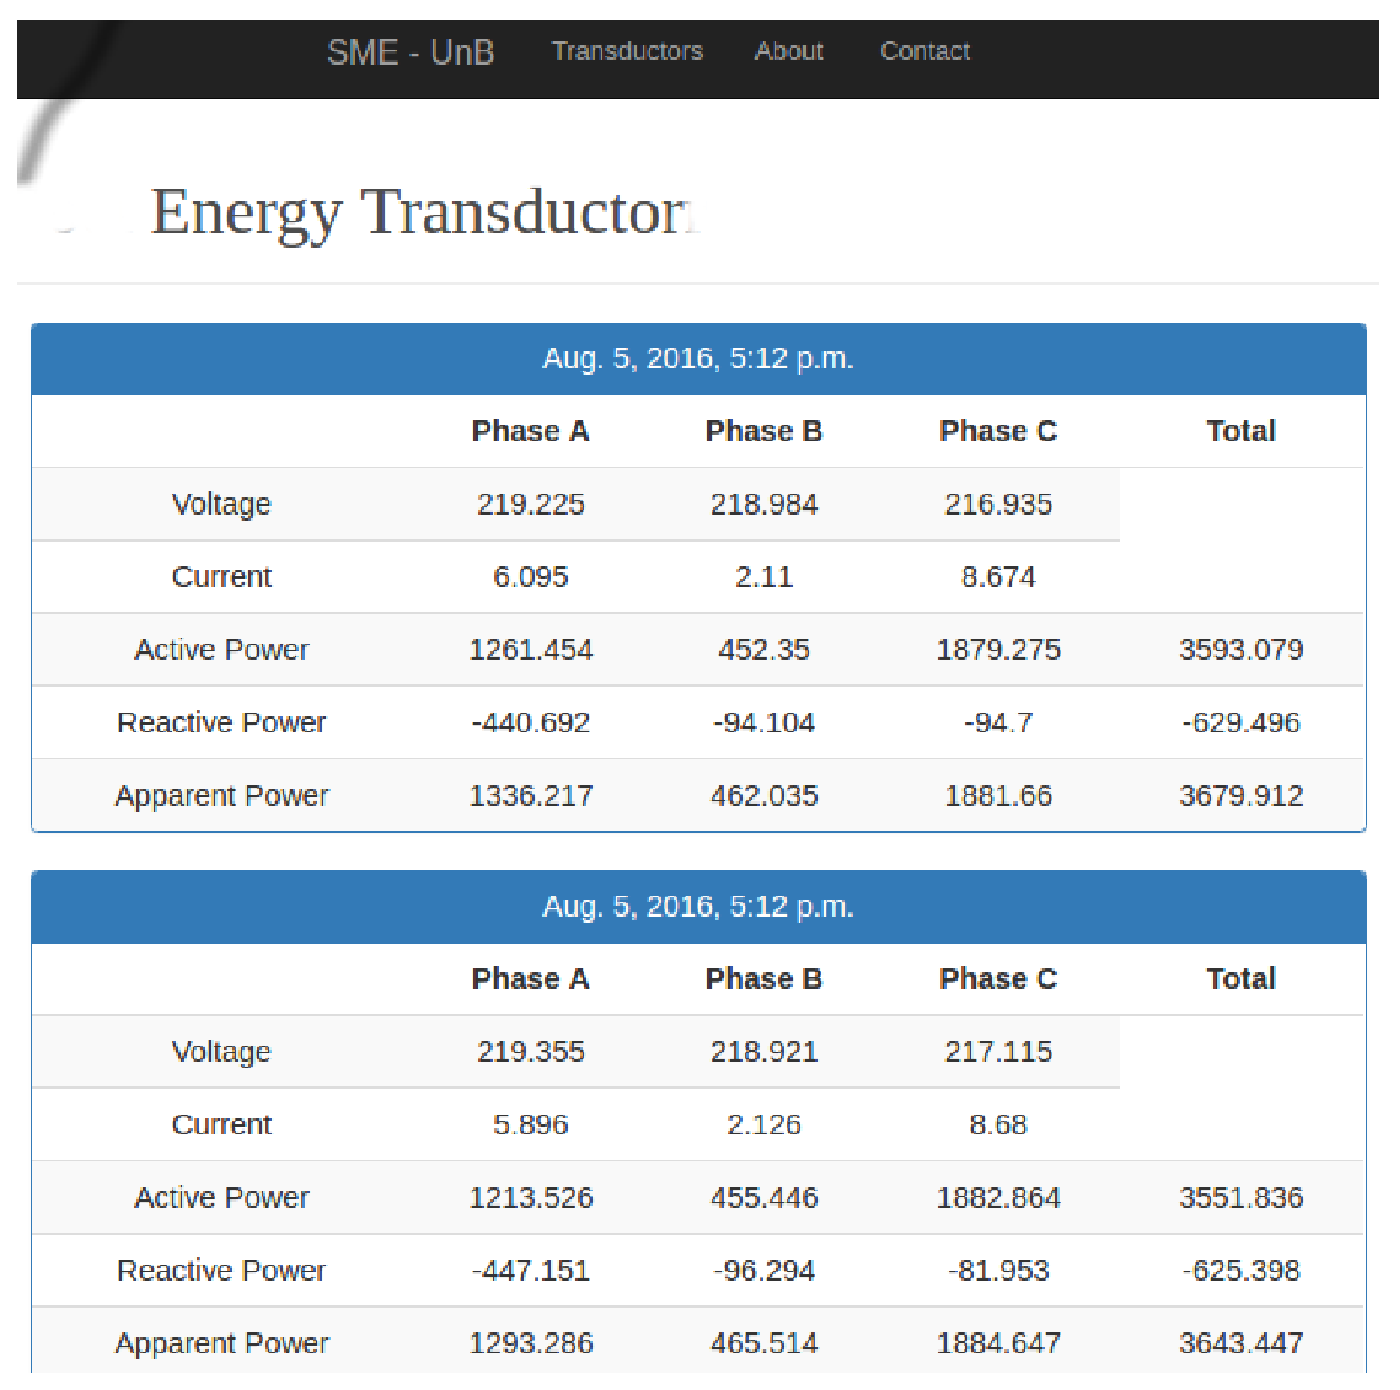
\includegraphics[keepaspectratio=true,scale=0.5]{figuras/coleta_dados_01.eps}
    \caption{Protótipo para apresentação de medições de energia \textit{release} 1.}
    \label{dados01}
\end{figure}

Foi realizado um guia de instalação para o ambiente de desenvolvimento no repositório. Esse guia objetiva tornar mais acessível o projeto a programadores que estivessem dispostos a realizar novas contribuições.

Uma vez que o código estava sendo escrito na linguagem Python 2.7, o desenvolvimento do projeto foi guiado pela utilização de suas boas práticas de programação, definidas pela PEP 8\footnote{\url{https://www.python.org/dev/peps/pep-0008/}}. Essas práticas buscam deixar o código mais legível e proporcionar uma maior eficiência, pois identificam problemas de indentação de código, tamanho de caracteres em uma linha, linhas em banco desnecessárias, bibliotecas importadas múltiplas vezes e outros padrões de estilo. A ferramenta utilizada para realizar a verificação dessas normas foi o flake8\footnote{\url{https://pypi.python.org/pypi/flake8}}.

Diversos testes unitários foram realizados a cada término de uma funcionalidade, objetivando uma cobertura de no mínimo 90\%. Os testes foram escritos utilizando o módulo \textit{unittest} do próprio Python. Esse ciclo de desenvolvimento permitiu identificar e corrigir pequenos erros de funcionalidades.

Utilizou-se a biblioteca \textit{mock}\footnote{\url{https://pypi.python.org/pypi/mock}}, do \textit{unittest}\footnote{\url{https://docs.python.org/3/library/unittest.html}}, para que fosse possível definir determinados comportamentos em métodos que utilizassem um outro método durante sua execução, objetivando um maior desempenho na hora de executar a suíte de testes e unitariedade dos métodos. A cobertura total de código obtida ao fim da \textit{release} 1 foi de 95\%, com 86 casos de teste.

Com o auxílio do serviço Gitlab CI, foi possível realizar de maneira fácil a integração contínua do projeto. Esse serviço utiliza como princípio um \textit{Runner}, que se baseia em uma máquina virtual isolada, responsável por realizar um \textit{Job}. Um \textit{Job} consiste na execução de comandos pré-definidos no arquivo padrão \textit{.gitlab-ci.yml}.

Diversas decisões arquiteturais e tecnológicas foram realizadas no decorrer da \textit{release} conforme as necessidades de implementação iam surgindo, objetivando modularizar e trazer maior robustez ao sistema. Uma delas foi a utilização da ferramenta \verb|cron|, objetivando realizar uma coleta de dados temporizada e autônoma das medições de energia.

Um ponto importante a se destacar, referente à primeira \textit{release}, é o da colaboração provinda por alunos de duas disciplinas aplicadas pelo curso de Engenharia de \textit{Software} na Faculdade  UnB Gama: Gestão de Projetos e Portfólio de \textit{Software} e Métodos de Desenvolvimento de \textit{Software}. As disciplinas em questão eram interdependentes e foram realizadas em conjunto.

O autor do trabalho atuou como \textit{Product Owner} \cite{scrum_guide} para as equipes, definindo os requisitos que deveriam ser feitos por elas. O \textit{Product Owner} (PO), ou dono do produto, é o responsável por maximizar o valor do produto e do trabalho do Time de Desenvolvimento realizando o gerenciamento do \textit{Backlog} do Produto\footnote{Lista com todas as funcionalidades desejadas para um produto.}. Os requisitos acordados com as equipes foram refentes à gerência de usuários, autenticação, geração de relatórios, \textit{log} para o sistema, sistema de alarme para eventos indesejados e autenticação na aplicação. Nem todos os requisitos foram realizados e os incrementos de \textit{software} providenciados ao projeto foram, em sua grande parte, referentes ao gerenciamento de usuários e autenticação.

\subsection{\textit{Release} 2}
A segunda \textit{release} teve início com uma forte refatoração sobre os incrementos de \textit{software} provindos das equipes de GPP e MDS. Em conjunto, visto que o projeto estava em Python 2.7, foi realizada uma mudança para Python 3.5. Junto a essa mudança, algumas modificações se concretizaram na autenticação do sistema, buscando que essa fosse realizada por meio de e-mail, em vez de nome de usuário.

Foi realizado um novo \textit{layout} para o sistema, visto que seria mais agradável ao usuário acessar páginas com cores agradáveis, botões significativos, perguntas de confirmação para ações importantes, \textit{links} para páginas anteriores e afins.

A apresentação periódica das informações energéticas se deve através de um gráfico de linhas dinâmico, com opções de aproximação e movimentação, para que o usuário pudesse visualizar pequenas ou longas faixas de medição. A biblioteca utilizada para realizar o gráfico foi a Matplotlib\footnote{\url{https://matplotlib.org/}}. Foram realizadas 3 opções para geração de gráfico, sendo estas:

\begin{itemize}
    \item Medições de Hoje: gera um gráfico de 00:00 até o horário atual;
    \item Medições de Dias Anteriores: é escolhido um, entre os 7 dias anteriores, para que seu gráfico possa ser gerado;
    \item Inserir Data Manualmente: um gráfico é gerado com base em uma data final e inicial. O período máximo definido entre as datas foi de 1 semana.
\end{itemize}

Com a expansão da aplicação, foi necessário realizar algumas mudanças para os usuários. A primeira mudança foi referente aos diferentes níveis de acesso, sendo permitido a criação de usuários administradores e normais. A criação dos usuários da aplicação só pode ser realizada por administradores, que possuem acesso sobre essa. A segunda mudança foi relacionada às permissões dos usuários normais, referentes à gerência de prédios ou transdutores. Essa gerências garantem os direitos de incluir, alterar, habilitar e desabilitar suas entidades.

Foi realizada uma API aberta que se comunica com algum sistema externo e expõe as informações de prédios, trandutores e medições de energia. Essa API é fundamental para o funcionamento do projeto, pois foi definido que toda gerência das entidades da aplicação será realizada na administração central.

O protótipo para comunicação entre uma administração central e os \textit{campi} da UnB foi realizado e utiliza a API anteriomente citada. Nesse protótipo dois tipos de sincronização são realizadas: sincronia de entidades e de medições. A sincronia de entidades é realizada quando se tenta cadastrar, por exemplo, um transdutor de um prédio presente em um determinado campus. Esse cadastro é concretizado apenas se houver uma comunicação entre o servidor da administração central e o servidor desse prédio. A sincronia de medições é feita quando a administração central extrai as últimas medições realizadas por cada prédio cadastrado.

Muitos testes unitários foram realizados nessa \textit{release}, objetivando cobrir as funcionalidades implementadas. Não foi possível realizar os testes para a API, pelo período de desenvolvimento ter chegado ao fim. A cobertura total de código obtida foi de 93\% e foram realizados 106 casos de teste a mais para a aplicação.

\section{Implantação}
Não foi possível colocar o SMI-UnB em produção, visto que muitas funcionalidades importantes ainda precisam ser desenvolvidas, porém, algumas de suas funções importantes foram implementadas com sucesso.

Alguns conhecimento provindos pelo \textit{Devops} foram utilizados para auxiliar na distribuição do SMI-UnB. O \textit{Devops} é um processo de desenvolvimento de \textit{software} que valoriza comunicação e colaboração entre gerentes de produto, desenvolvedores de \textit{software} e outros profissionais. O \textit{DevOps} também automatiza os processos de integração de \textit{software}, testes, implantação e mudanças de infraestrutura \cite{loukides_2012}.

Utilizou-se o Docker\footnote{\url{https://www.docker.com/}} para que fosse possível criar um ambiente unificado para o sistema, visando evitar futuros problemas de implantação.

O Docker é uma plataforma de contêiners de \textit{software}. Um contêiner, Figura \ref{container}, possui empacotado tudo que é necessário para se executar um \textit{software} completo ou parte dele. Diferente das máquinas virtuais, os contêiners são executados em uma mesma máquina, compartilhando o \textit{kernel} do seu sistema operacional, sendo que cada um terá seu processo isolado no espaço de usuário.

\begin{figure}[!h]
    \centering
    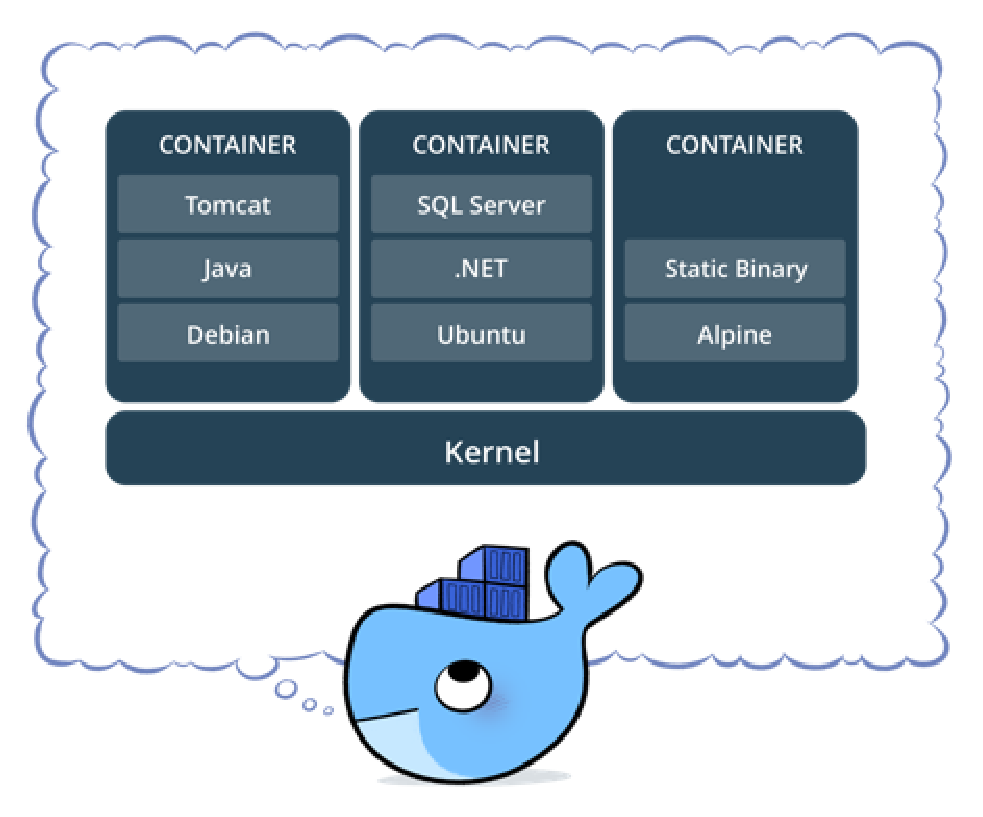
\includegraphics[keepaspectratio=true,scale=0.8]{figuras/container.eps}
    \caption{Exemplo de contêiners providos pelo Docker. Fonte: \cite{docker} }
    \label{container}
\end{figure}

Para Tanenbaum \cite{tanenbaum_2007}, o sistema operacional é a peça mais básica de \textit{software} e opera em modo núcleo, possuindo acesso completo a todo o \textit{hardware} e ao conjunto de instruções oferecidos pela máquina. O resto do \textit{software} opera em modo usuário, onde é disponível apenas um conjunto de instruções da máquina para execução.

Realizou-se um ambiente para testes no campus UnB-Gama, que possuía o SMI-UnB instalado como um serviço, objetivando averiguar o que havia sido implementado.